\chapter{Erstellen eines Projekts}
\label{ch:erstellen_eines_projekts}

Liegt noch kein Projekt in Form einer >>.gm<< Datei vor, so muss dies erst erstellt werden. Dazu starten sie das Programm wie es in Kapitel \ref{ch:installation} erklärt wurde. Nun wechseln sie in den Bearbeitungsmodus. Sie sehen in der Arbeitsfläche ein leeres Textfeld. Dort müssen sie nun ihre Gruppen und Personen in der >>.gm<< Syntax eintragen, was im Folgenden Abschnitt erklärt wird.

\section{Die >>.gm<< Syntax}
\label{sec:die_>>.gm<<_syntax}

Hier wird erklärt, wie eine >>.gm<< Datei aufgebaut ist. In der folgenden Weise werden nicht nur >>GroupMatcher<< Projekte gespeichert, sondern auch vom Benutzer erstellt. Dank dem einfachen Aufbau ist die Syntax schnell erlernt und dann ist sie wesentlich effektiver als jede graphische Lösung der Bearbeitung. Um die folgende Erläuterung besser zu verstehen, kann zum einen Abbildung \ref{fig:die_syntax} mit der theoretischen Syntax \mnote{In der theoretischen Syntax gelten Folgende Regeln:\\
	- in spitze Klammern (<>) eingeschlossene Wörter stellen Variablen dar\\
	- in eckige Klammern ([]) eingeschlossene Gefüge sind optional\\
	- drei Punkte (...) stehen für eine unbegrenzte Wiederholung des davor stehenden Gefüges
} und zum anderen Abbildung \ref{fig:ein_beispiel} mit einem Beispielcode helfen.

\begin{figure}
	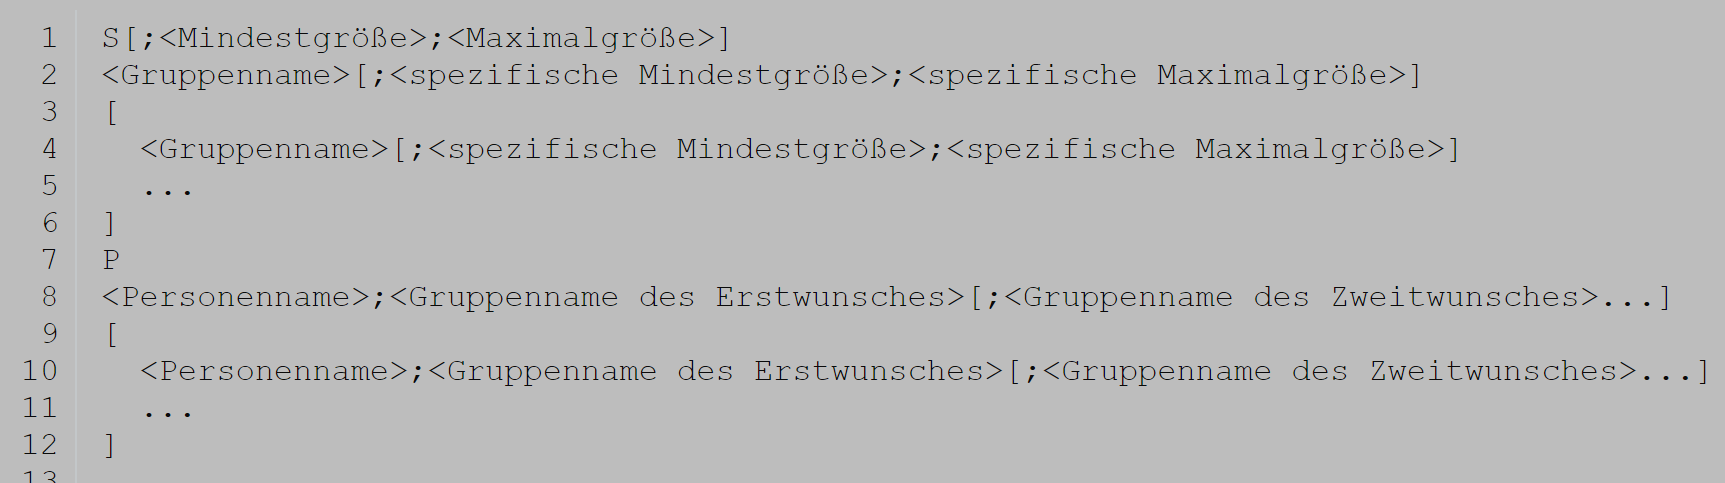
\includegraphics{syntax}
	\caption{Die Syntax der >>.gm<< Dateien}
	\label{fig:die_syntax}
\end{figure}

\begin{figure}
	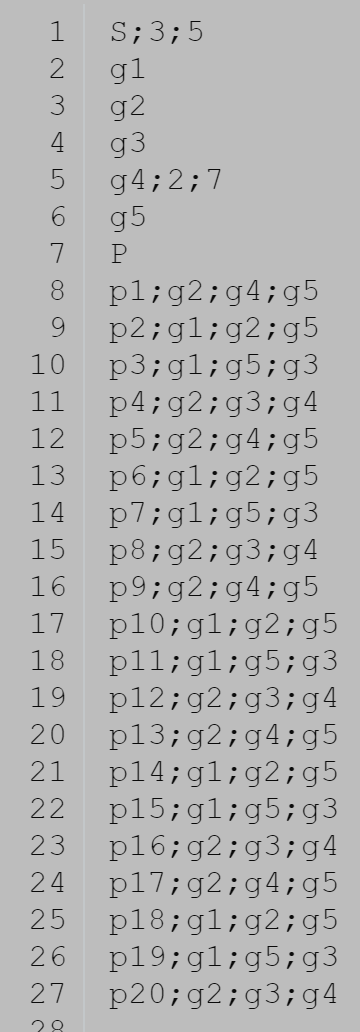
\includegraphics[width=3cm]{beispiel}
	\caption{Ein Beispiel einer >>.gm<< Datei}
	\label{fig:ein_beispiel}
\end{figure}

\paragraph{Gruppendeklaration} Am Anfang der Datei steht der \hl{Gruppenindikator} >>S<<. Dieser zeigt dem Übersetzerprogramm an, dass nun die Informationen für Gruppen folgen. In der Zeile des Gruppenindikators können durch Semikolons \mnote{Semikolon = ;} getrennt eine \hl{allgemeine Mindest- und Maximalgröße} festgelegt werden. Diese gilt dann für alle Gruppen, für die nicht später eigenen Werte festgelegt werden. Wird kein allgemeiner Wert festgelegt, so wird für beide Werte der Wert 0 angenommen.\\
Ab der darauffolgenden Zeile können Gruppen definiert werden. Dabei steht immer am Anfang der Zeile der \hl{Gruppenname}. Soll für die Gruppen nicht die allgemein definierten Werte für Mindest- und Maximalgröße gelten, so können wiederum durch Semikolons getrennt die \hl{spezielle Mindest- und Maximalgröße} festgelegt werden. In jeder Zeile darf dabei immer nur eine Gruppe stehen.
\paragraph{Personendeklaration} Sind alle Gruppen definiert, so folgt in der nächsten Zeile der \hl{Personenindikator} >>P<<.\\
Ab der nächsten Zeile können Personen definiert werden. Dabei steht am Anfang jeder Zeile der \hl{Personenname}, gefolgt von einem Semikolon. Danach kann, durch Semikolons separiert, eine unbegrenzte Anzahl \mnote{Auch wenn im Zuordnungsmodus der Benutzeroberfläche nur drei Wünsche angezeigt werden, unterstützt das Programm bei allen anderen Funktionen eine unbegrenzte Anzahl an Wünschen.}, aber mindestens ein Wunsch festgelegt werden. Dies geschieht durch das Nennen des \hl{Gruppennamens} der gewünschten Gruppe. Sind alle Wünsche festgelegt, so kann die Person einer seiner Wünsche zugeordnet werden, was aber für den Benutzer irrelevant ist, sondern nur beim Speichern des Projekts eine Rolle spielt, was aber vom Programm erledigt wird. Die Syntax dazu ist aber ein Schrägstrich gefolgt von dem Gruppennamen des erfüllten Wunsches. Pro Zeile darf wiederum nur eine Person deklariert werden.

\section{Abschließen des Erstellvorgangs}
\label{sec:abschliessen_des_erstellvorgangs}

Wurden alle Gruppen und Personen wie oben erklärt erstellt, so kann nun mit der Zuteilung begonnen werden. Dazu betätigen \mnote{Drücken sie auf zuordnen.} sie den Wechselschalter in der oberen rechten Ecke. Falls nun eine Fehlermeldung erscheint versuchen sie diese zu beheben. Dabei kann ihnen das Kapitel \ref{ch:fehlermeldungen} helfen. Ansonsten gelangen sie jetzt in den Zuordnungsmodus. Zugleich öffnet sich ein Dialog, der sie zum speichern des Projekts auffordert. Dies sollten sie nun unbedingt tun, da das Projekt verfällt, falls noch kein Speicherpfad angegeben ist, wenn das Programm geschlossen wird. Haben sie das Projekt erfolgreich gespeichert, so ist der Erstellvorgang abgeschlossen.
